\documentclass[11pt,letterpaper]{article}

\usepackage[margin=1in,headheight=14pt]{geometry}
\usepackage{amsmath,amssymb,amsthm}
\usepackage{algorithm}
\usepackage{algpseudocode}
\usepackage{listings}
\usepackage{xcolor}
\usepackage{hyperref}
\usepackage{tikz}
\usetikzlibrary{arrows.meta,positioning,shapes.geometric,fit,calc}
\usepackage{booktabs}
\usepackage{enumitem}
\usepackage{fancyhdr}
\usepackage{tcolorbox}
\usepackage{bytefield}

\tcbuselibrary{listingsutf8,skins}

\hypersetup{
    colorlinks=true,
    linkcolor=blue!70!black,
    citecolor=green!50!black,
    urlcolor=blue!60!black
}

\definecolor{codebg}{RGB}{248,248,248}
\definecolor{codeframe}{RGB}{200,200,200}
\definecolor{keyword}{RGB}{0,0,180}
\definecolor{comment}{RGB}{0,128,0}
\definecolor{string}{RGB}{180,0,0}

\lstdefinestyle{rust}{
    language=C,
    basicstyle=\ttfamily\small,
    keywordstyle=\color{keyword}\bfseries,
    commentstyle=\color{comment}\itshape,
    stringstyle=\color{string},
    backgroundcolor=\color{codebg},
    frame=single,
    rulecolor=\color{codeframe},
    breaklines=true,
    showstringspaces=false,
    tabsize=4,
    morekeywords={fn,let,mut,pub,struct,enum,impl,self,Self,match,use,mod,trait,const,u8,u16,u32,u64,i8,i16,i32,i64,usize,isize,bool,Vec,Option,Result,Some,None,Ok,Err}
}

\lstdefinestyle{asm}{
    basicstyle=\ttfamily\small,
    backgroundcolor=\color{codebg},
    frame=single,
    rulecolor=\color{codeframe},
    breaklines=true,
    showstringspaces=false,
    commentstyle=\color{comment}\itshape,
    morecomment=[l]{//},
    morecomment=[l]{\#},
}

\newtcolorbox{keyinsight}{
    colback=blue!5!white,
    colframe=blue!50!black,
    title=Key Insight,
    fonttitle=\bfseries
}

\newtcolorbox{definition}{
    colback=green!5!white,
    colframe=green!50!black,
    title=Definition,
    fonttitle=\bfseries
}

\newtcolorbox{warning}{
    colback=red!5!white,
    colframe=red!50!black,
    title=Important,
    fonttitle=\bfseries
}

\newtheorem{theorem}{Theorem}
\newtheorem{lemma}[theorem]{Lemma}
\newtheorem{proposition}[theorem]{Proposition}

\pagestyle{fancy}
\fancyhf{}
\rhead{NVMirror Technical Guide}
\lhead{\leftmark}
\cfoot{\thepage}

\title{\textbf{NVMirror: An eBPF Just-In-Time Compiler\\for NVMe Controller Processors}\\[0.5em]
\large A Complete Technical Guide for Researchers\\Without Compiler or Assembly Background}
\author{NVMirror Project}
\date{May 2026}

\begin{document}

\maketitle

\begin{abstract}
This document provides a self-contained explanation of the NVMirror project: a Just-In-Time (JIT) compiler that translates eBPF bytecode into native machine code for NVMe storage controller processors. We assume no prior knowledge of compilers, assembly language, or eBPF. Every concept is introduced from first principles with concrete examples. The document is structured so that a researcher in systems, networking, or storage can understand \emph{what} the system does, \emph{why} each design decision was made, and \emph{how} the implementation achieves provable correctness.
\end{abstract}

\tableofcontents
\newpage

%===========================================================================
\section{Background: What Problem Are We Solving?}
%===========================================================================

\subsection{The Storage Performance Gap}

Modern NVMe solid-state drives (SSDs) can deliver over 7~GB/s of bandwidth and millions of I/O operations per second. However, to \emph{process} the data read from storage, it must travel across a PCIe bus to the host CPU, be processed, and potentially travel back. This round-trip creates latency and consumes host CPU cycles and memory bandwidth.

\begin{keyinsight}
\textbf{Computational storage} moves computation \emph{into} the storage device itself. Instead of transferring data to the CPU for processing, we send a small program to the drive's internal processor and let it process data in-place, near the flash media.
\end{keyinsight}

\subsection{The Challenge: Running User Programs on Controller Firmware}

NVMe controllers contain small embedded processors (typically ARM Cortex-R or RISC-V cores). These processors run firmware---fixed software burned into the device. We want to allow users to send \emph{custom programs} that execute on this firmware, but with critical constraints:

\begin{enumerate}[label=(\arabic*)]
    \item \textbf{Safety}: A user program must not crash the controller, corrupt data, or access unauthorized memory.
    \item \textbf{Performance}: Programs must run at near-native speed, not through a slow software interpreter.
    \item \textbf{Resource limits}: The controller has limited RAM (often $<$1~MB), no virtual memory, and no operating system.
\end{enumerate}

This is where eBPF and JIT compilation enter the picture.

%===========================================================================
\section{Prerequisite Concepts}
%===========================================================================

\subsection{What Is a Processor Instruction?}

At the lowest level, a processor executes \emph{instructions}---fixed-width binary patterns that encode operations. For example, on an ARM processor, the 32-bit pattern:

\begin{center}
\texttt{0xD2800547}
\end{center}

\noindent means ``place the number 42 into register X7.'' Every program you have ever run---from a web browser to a database---ultimately reduces to a sequence of such binary instructions.

\begin{definition}
A \textbf{register} is a tiny, ultra-fast storage cell inside the processor. A typical processor has 16--32 registers, each holding one 64-bit integer. All arithmetic, logic, and data movement operations work on registers.
\end{definition}

\subsection{What Is Assembly Language?}

Assembly language is a human-readable notation for binary instructions. Instead of writing \texttt{0xD2800547}, we write:

\begin{lstlisting}[style=asm]
MOVZ X7, #42      // Load the immediate value 42 into register X7
\end{lstlisting}

\noindent There is a one-to-one correspondence between assembly mnemonics and binary machine code. An \emph{assembler} translates the text form to binary; a \emph{disassembler} does the reverse.

\subsection{What Is a Compiler?}

A compiler translates a program from one language (the \emph{source}) to another (the \emph{target}). Typically:
\begin{itemize}
    \item A C compiler translates C source code into machine code for x86 or ARM.
    \item The translation happens \emph{before} the program runs (\textbf{ahead-of-time} compilation).
\end{itemize}

\subsection{What Is a Just-In-Time (JIT) Compiler?}

\begin{definition}
A \textbf{Just-In-Time compiler} translates a program into machine code \emph{at runtime}, immediately before executing it. The source is typically a portable \emph{bytecode} format (not human-readable source code).
\end{definition}

The key advantage: the input bytecode is portable (runs on any target), but execution speed equals native machine code because we compile it to the specific processor's instruction set just before running it.

\begin{center}
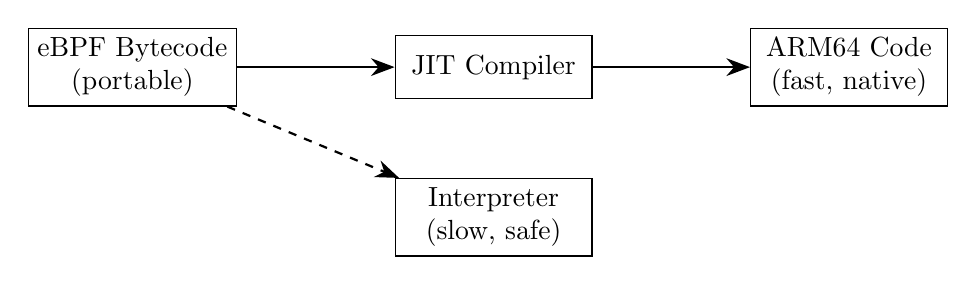
\begin{tikzpicture}[
    box/.style={rectangle, draw, minimum width=2.5cm, minimum height=0.8cm, align=center},
    arrow/.style={-{Stealth[length=3mm]}, thick}
]
\node[box] (src) {eBPF Bytecode\\(portable)};
\node[box, right=2cm of src] (jit) {JIT Compiler};
\node[box, right=2cm of jit] (native) {ARM64 Code\\(fast, native)};
\node[box, below=1cm of jit] (interp) {Interpreter\\(slow, safe)};

\draw[arrow] (src) -- (jit);
\draw[arrow] (jit) -- (native);
\draw[arrow, dashed] (src) -- (interp);
\end{tikzpicture}
\end{center}

\subsection{What Is eBPF?}

\begin{definition}
\textbf{eBPF} (extended Berkeley Packet Filter) is a virtual instruction set architecture (ISA) originally designed for safely filtering network packets inside the Linux kernel. It defines a simple, restricted virtual machine with:
\begin{itemize}
    \item 11 registers (R0--R10), each 64 bits wide
    \item A 512-byte stack
    \item No loops (programs must terminate)
    \item No arbitrary memory access (all pointers are bounds-checked)
\end{itemize}
\end{definition}

eBPF was designed to be \emph{statically verifiable}---a program's safety can be proven \emph{before} execution, without running it. This is what makes it ideal for untrusted code on embedded controllers.

\subsubsection{eBPF Instruction Encoding}

Each eBPF instruction is exactly 8 bytes (64 bits) with this layout:

\begin{center}
\begin{bytefield}[bitwidth=1.2em]{64}
\bitheader{0,7,8,11,12,15,16,31,32,63} \\
\bitbox{8}{opcode} & \bitbox{4}{dst} & \bitbox{4}{src} & \bitbox{16}{offset} & \bitbox{32}{immediate}
\end{bytefield}
\end{center}

\begin{itemize}
    \item \textbf{opcode} (8 bits): Encodes the operation class and specific operation.
    \item \textbf{dst} (4 bits): Destination register number (0--10).
    \item \textbf{src} (4 bits): Source register number (0--10).
    \item \textbf{offset} (16 bits, signed): Memory offset for load/store, or branch displacement.
    \item \textbf{immediate} (32 bits, signed): Constant operand.
\end{itemize}

\subsubsection{eBPF Instruction Classes}

The low 3 bits of the opcode determine the instruction \emph{class}:

\begin{center}
\begin{tabular}{ccl}
\toprule
\textbf{Class} & \textbf{Bits [2:0]} & \textbf{Description} \\
\midrule
ALU & \texttt{0x04} & 32-bit arithmetic/logic \\
ALU64 & \texttt{0x07} & 64-bit arithmetic/logic \\
JMP & \texttt{0x05} & 64-bit conditional/unconditional jumps \\
JMP32 & \texttt{0x06} & 32-bit conditional jumps \\
LD & \texttt{0x00} & Load from packet/immediate \\
LDX & \texttt{0x01} & Load from memory \\
ST & \texttt{0x02} & Store immediate to memory \\
STX & \texttt{0x03} & Store register to memory \\
\bottomrule
\end{tabular}
\end{center}

\subsubsection{Example: A Minimal eBPF Program}

Consider a program that returns the number 42:

\begin{lstlisting}[style=asm]
MOV64 R0, 42    // R0 = 42 (return value register)
EXIT            // End program, return R0 to caller
\end{lstlisting}

Encoded as raw bytes (two 8-byte instructions):
\begin{lstlisting}[style=asm]
B7 00 00 00 2A 00 00 00    // opcode=0xB7 (ALU64|MOV|K), dst=R0, imm=42
95 00 00 00 00 00 00 00    // opcode=0x95 (JMP|EXIT)
\end{lstlisting}

\subsection{What Is an Instruction Set Architecture (ISA)?}

\begin{definition}
An \textbf{ISA} is the contract between software and hardware. It specifies:
\begin{itemize}
    \item What instructions exist (ADD, MUL, LOAD, BRANCH, etc.)
    \item How many registers are available and how wide they are
    \item How instructions are encoded in binary
    \item How memory is addressed
\end{itemize}
\end{definition}

NVMirror targets two ISAs:
\begin{itemize}
    \item \textbf{AArch64} (ARM 64-bit): Used in Apple M-series chips, NVIDIA Jetson, and ARM Cortex-R82 NVMe controllers. Instructions are fixed at 32 bits wide.
    \item \textbf{RISC-V RV64}: An open-source ISA used in emerging NVMe controllers. Base instructions are 32 bits wide.
\end{itemize}

\subsection{What Is NVMe?}

NVMe (Non-Volatile Memory Express) is the standard interface protocol for SSDs connected via PCIe. An NVMe controller is the embedded system inside the SSD that manages flash memory, handles I/O commands, and now (with NVMirror) can execute computational programs.

%===========================================================================
\section{System Architecture}
%===========================================================================

NVMirror is structured as a \textbf{multi-stage pipeline}. Each stage transforms the program into a representation closer to executable machine code, while maintaining safety invariants.

\begin{center}
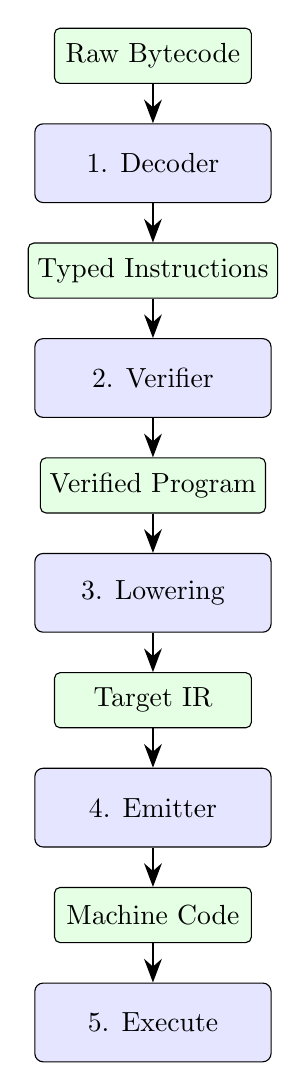
\begin{tikzpicture}[
    stage/.style={rectangle, draw, fill=blue!10, minimum width=3cm, minimum height=1cm, align=center, rounded corners=3pt},
    data/.style={rectangle, draw, fill=green!10, minimum width=2.5cm, minimum height=0.7cm, align=center, rounded corners=2pt},
    arrow/.style={-{Stealth[length=3mm]}, thick},
    node distance=0.5cm
]
\node[data] (raw) {Raw Bytecode};
\node[stage, below=of raw] (decode) {1. Decoder};
\node[data, below=of decode] (insns) {Typed Instructions};
\node[stage, below=of insns] (verify) {2. Verifier};
\node[data, below=of verify] (verified) {Verified Program};
\node[stage, below=of verified] (lower) {3. Lowering};
\node[data, below=of lower] (ir) {Target IR};
\node[stage, below=of ir] (emit) {4. Emitter};
\node[data, below=of emit] (code) {Machine Code};
\node[stage, below=of code] (exec) {5. Execute};

\draw[arrow] (raw) -- (decode);
\draw[arrow] (decode) -- (insns);
\draw[arrow] (insns) -- (verify);
\draw[arrow] (verify) -- (verified);
\draw[arrow] (verified) -- (lower);
\draw[arrow] (lower) -- (ir);
\draw[arrow] (ir) -- (emit);
\draw[arrow] (emit) -- (code);
\draw[arrow] (code) -- (exec);
\end{tikzpicture}
\end{center}

%===========================================================================
\section{Stage 1: Decoding}
\label{sec:decoder}
%===========================================================================

\subsection{Purpose}

The decoder (\texttt{crates/ebpf-core/src/decode.rs}) transforms raw 8-byte instruction encodings into a \emph{strongly typed} Rust data structure. This is analogous to parsing---converting an unstructured byte stream into a structured abstract syntax tree.

\subsection{Why Strong Typing Matters}

In the raw encoding, a register number is just 4 bits that could contain any value from 0 to 15. But eBPF only has registers 0--10. By parsing into a \texttt{BpfReg} type that \emph{rejects} values above 10 at construction time, we make invalid register references \textbf{unrepresentable} in our program. This is a form of \emph{correct-by-construction} design:

\begin{lstlisting}[style=rust]
pub struct BpfReg(u8);  // Invariant: self.0 <= 10

impl BpfReg {
    pub const fn from_raw(raw: u8) -> Option<Self> {
        if raw <= 10 { Some(Self(raw)) } else { None }
    }
}
\end{lstlisting}

After decoding, every subsequent stage can assume all register references are valid without re-checking.

\subsection{Decoded Instruction Format}

The decoder produces a Rust \texttt{enum} (sum type) where each variant represents exactly one kind of eBPF instruction with precisely the operands it needs:

\begin{lstlisting}[style=rust]
enum Insn {
    Alu64 { op: AluOp, dst: BpfReg, src: Source },
    Load  { width: MemWidth, dst: BpfReg, src: BpfReg, off: i16 },
    JmpCond { op: JmpOp, dst: BpfReg, src: Source, off: i16 },
    Exit,
    // ... other variants
}
\end{lstlisting}

\subsection{Algorithmic Complexity}

The decoder performs a single linear scan over the instruction array:
\[
T(\text{decode}) = O(n) \quad \text{where } n = \text{number of instructions}
\]

The only special case is the 64-bit immediate load (LDDW), which consumes two consecutive 8-byte slots to encode a full 64-bit constant.

%===========================================================================
\section{Stage 2: Verification}
\label{sec:verifier}
%===========================================================================

\subsection{Purpose}

The verifier (\texttt{crates/ebpf-core/src/verify.rs}) is the \textbf{safety critical} component. It statically proves that the program cannot:
\begin{enumerate}
    \item Read an uninitialized register (undefined behavior)
    \item Write to R10 (the read-only frame pointer)
    \item Branch outside the program's instruction array
    \item Access stack memory outside the 512-byte frame
    \item Fail to terminate (infinite loops)
    \item Contain dead/unreachable code (potential confusion)
\end{enumerate}

\begin{warning}
If the verifier accepts a program, all subsequent stages can \emph{assume} these properties hold without rechecking. A bug in the verifier compromises the entire system's safety. This is why it is the most heavily tested component.
\end{warning}

\subsection{Control-Flow Graph Construction}

The verifier first builds a \textbf{Control-Flow Graph (CFG)}---a directed graph where:
\begin{itemize}
    \item \textbf{Nodes} are basic blocks (maximal sequences of instructions with no internal branches).
    \item \textbf{Edges} represent possible flow: fall-through to the next block, or a branch to a target block.
\end{itemize}

\begin{definition}
A \textbf{basic block} is a sequence of instructions where:
\begin{enumerate}
    \item The only entry point is the first instruction (no jumps into the middle).
    \item The only exit point is the last instruction (which is either a branch, return, or falls through to the next block).
\end{enumerate}
\end{definition}

New basic blocks start at:
\begin{itemize}
    \item The program entry point (instruction 0)
    \item Any instruction that is the target of a branch
    \item Any instruction immediately following a branch or exit
\end{itemize}

\subsection{Dataflow Analysis: Register Initialization Tracking}

The verifier performs a \textbf{fixed-point dataflow analysis} to track which registers are initialized at each point in the program.

\subsubsection{Lattice}

Each register has a state from the lattice $\{$\textsc{Uninit}, \textsc{Init}$\}$. At the program entry:
\begin{itemize}
    \item R1 = \textsc{Init} (context pointer, provided by the caller)
    \item R10 = \textsc{Init} (frame pointer, always valid)
    \item R0, R2--R9 = \textsc{Uninit}
\end{itemize}

\subsubsection{Transfer Functions}

For each instruction, we update the register state:
\begin{itemize}
    \item \texttt{MOV R3, 42}: Sets R3 $\to$ \textsc{Init}
    \item \texttt{ADD R0, R1}: Reads R0 and R1 (must both be \textsc{Init}), result in R0 remains \textsc{Init}
    \item \texttt{CALL helper}: R0 $\to$ \textsc{Init} (return value), R1--R5 $\to$ \textsc{Uninit} (clobbered)
\end{itemize}

\subsubsection{Merge at Join Points}

When two control-flow paths converge (e.g., after an if/else), register states are merged conservatively:
\[
\text{merge}(s_1, s_2) = \begin{cases} \textsc{Init} & \text{if } s_1 = \textsc{Init} \wedge s_2 = \textsc{Init} \\ \textsc{Uninit} & \text{otherwise} \end{cases}
\]

This means: a register is considered initialized at a merge point \emph{only if} it is initialized on \emph{all} incoming paths.

\subsubsection{Convergence}

The analysis iterates until no register states change (fixed point). Since the lattice has only two elements and states can only go from \textsc{Init} $\to$ \textsc{Uninit} (never the reverse) at merge points, convergence is guaranteed in at most $O(k)$ iterations where $k$ is bounded by the number of back-edges (loops). eBPF programs have bounded loops, so:
\[
T(\text{verify}) = O(n \cdot k), \quad k \leq 32
\]

\subsection{Stack Bounds Checking}

When an instruction accesses memory relative to R10 (the frame pointer), the verifier checks:
\[
-512 \leq \text{offset} < 0
\]

The eBPF stack grows downward from R10. Any access at offset $\geq 0$ or $< -512$ is rejected.

%===========================================================================
\section{Stage 3: Lowering and Register Allocation}
\label{sec:regalloc}
%===========================================================================

\subsection{Purpose}

Lowering (\texttt{crates/jit-regalloc/src/lib.rs}) transforms verified eBPF instructions into a \textbf{target-independent intermediate representation (IR)} that uses \emph{physical registers} instead of virtual eBPF registers.

\subsection{The Register Allocation Problem}

eBPF programs use virtual registers R0--R10. The target processor has \emph{physical} registers (X0--X30 on AArch64, x0--x31 on RISC-V). We must decide which physical register holds each virtual register's value.

\begin{definition}
\textbf{Register allocation} is the process of assigning virtual registers to physical registers. When there are more virtual registers than physical registers, some values must be \emph{spilled} to memory (the stack) and later \emph{filled} (reloaded).
\end{definition}

\subsection{Our Strategy: Fixed Mapping}

Since eBPF has only 11 registers and both target ISAs have $>$30, we use a \textbf{fixed, predetermined mapping}---no complex allocation algorithm needed:

\begin{center}
\begin{tabular}{ccc}
\toprule
\textbf{eBPF Register} & \textbf{AArch64} & \textbf{RISC-V} \\
\midrule
R0 (return value) & X7 & a0 \\
R1 (argument 1) & X0 & a1 \\
R2 (argument 2) & X1 & a2 \\
R3 (argument 3) & X2 & a3 \\
R4 (argument 4) & X3 & a4 \\
R5 (argument 5) & X4 & a5 \\
R6 (callee-saved) & X19 & s2 \\
R7 (callee-saved) & X20 & s3 \\
R8 (callee-saved) & X21 & s4 \\
R9 (callee-saved) & X22 & s5 \\
R10 (frame pointer) & X25 & s6 \\
\midrule
Scratch/temp & X9 & s7 \\
\bottomrule
\end{tabular}
\end{center}

\begin{keyinsight}
The AArch64 mapping places eBPF R1--R5 in X0--X4. This is deliberate: when our JIT'd code calls a helper function, the arguments are already in the correct registers per the ARM calling convention, avoiding any register shuffling. This zero-cost ABI alignment is a significant performance optimization.
\end{keyinsight}

\subsection{Callee-Saved Registers and the Prologue/Epilogue}

\begin{definition}
In a \textbf{calling convention}, some registers are designated \textbf{callee-saved}: if a function modifies them, it must restore their original values before returning. Other registers are \textbf{caller-saved}: the caller assumes they may be destroyed by any function call.
\end{definition}

On AArch64, X19--X28 are callee-saved. Since eBPF R6--R9 map to X19--X22, any program that writes to R6--R9 must:
\begin{enumerate}
    \item \textbf{Prologue}: Save the original X19--X22 values to the stack at function entry.
    \item \textbf{Epilogue}: Restore them from the stack before returning.
\end{enumerate}

The lowering pass detects whether any instruction writes to R6--R9 and, if so, emits Prologue/Epilogue IR nodes.

\subsection{The IR (Intermediate Representation)}

The IR (\texttt{crates/jit-ir/src/lib.rs}) uses the same instruction \emph{kinds} as eBPF but with physical registers and explicit basic-block labels:

\begin{lstlisting}[style=rust]
enum IrNode {
    Alu64 { op: AluOp, dst: PhysReg, src: Operand },
    Load  { width: MemWidth, dst: PhysReg, base: PhysReg, off: i16 },
    Branch { cond: BranchCond, target: BasicBlockId },
    Jump { target: BasicBlockId },
    Prologue { frame_size: u16 },
    Epilogue { frame_size: u16 },
    Ret,
    // ...
}
\end{lstlisting}

Branch targets are \texttt{BasicBlockId} values (indices into an array), not raw byte offsets. This makes out-of-bounds jumps \emph{structurally impossible}---you cannot construct an \texttt{IrNode::Branch} pointing to a nonexistent block.

%===========================================================================
\section{Stage 4: Code Emission}
\label{sec:emission}
%===========================================================================

\subsection{Purpose}

The emitter translates each IR node into one or more \emph{binary-encoded} target instructions. NVMirror has two emitters:
\begin{itemize}
    \item \texttt{crates/jit-aarch64/}: Emits ARM AArch64 machine code
    \item \texttt{crates/jit-riscv/}: Emits RISC-V RV64IMC machine code
\end{itemize}

\subsection{Instruction Encoding: AArch64 Example}

On AArch64, every instruction is exactly 32 bits (4 bytes). The encoding packs the operation and operands into specific bit fields. For example, \texttt{ADD X7, X7, X9}:

\begin{center}
\begin{bytefield}[bitwidth=0.9em]{32}
\bitheader{0,4,5,9,10,15,16,20,21,28,29,30,31} \\
\bitbox{1}{1} & \bitbox{2}{00} & \bitbox{6}{01011} & \bitbox{3}{000} & \bitbox{5}{01001} & \bitbox{6}{000000} & \bitbox{5}{00111} & \bitbox{5}{00111}
\end{bytefield}
\end{center}

\begin{itemize}
    \item Bit 31 (sf=1): 64-bit operation
    \item Bits 30--29 (op=00): ADD (not SUB)
    \item Bits 28--24: Fixed encoding for ``data processing, register''
    \item Bits 20--16 (Rm=01001): Second source register X9
    \item Bits 9--5 (Rn=00111): First source register X7
    \item Bits 4--0 (Rd=00111): Destination register X7
\end{itemize}

The emitter functions encode this as pure arithmetic:
\begin{lstlisting}[style=rust]
pub const fn add_x_reg(rd: u8, rn: u8, rm: u8) -> u32 {
    0x8B000000 | ((rm as u32) << 16) | ((rn as u32) << 5) | (rd as u32)
}
\end{lstlisting}

\subsection{Handling Immediate Values}

eBPF instructions can have 64-bit immediates, but AArch64 instructions only have room for 12--16 bits of immediate data. To load a full 64-bit constant, we must use a multi-instruction sequence:

\begin{lstlisting}[style=asm]
MOVZ X7, #0x5678           // X7 = 0x0000_0000_0000_5678
MOVK X7, #0x1234, LSL #16  // X7 = 0x0000_0000_1234_5678
MOVK X7, #0xABCD, LSL #32  // X7 = 0x0000_ABCD_1234_5678
MOVK X7, #0x9999, LSL #48  // X7 = 0x9999_ABCD_1234_5678
\end{lstlisting}

\texttt{MOVZ} loads a 16-bit value and zeros the rest. Each subsequent \texttt{MOVK} ``keeps'' the existing bits and inserts 16 new bits at the specified position. The emitter optimizes this by omitting \texttt{MOVK} for zero chunks.

\subsection{Branch Handling and Relocations}

Branches pose a challenge: when emitting a branch instruction, we may not yet know the \emph{byte offset} of the target basic block (it hasn't been emitted yet). The solution:

\begin{enumerate}
    \item Emit the branch with a \textbf{placeholder} offset of zero.
    \item Record a \textbf{relocation}: ``at byte offset $X$ in the buffer, patch in the offset to basic block $B$.''
    \item After all blocks are emitted, \textbf{finalize}: walk the relocation table and patch each branch with the now-known target offset.
\end{enumerate}

\begin{lstlisting}[style=rust]
struct Relocation {
    offset: usize,        // Where in the buffer the branch lives
    target: BasicBlockId, // Which BB it should jump to
    is_conditional: bool, // B.cond (19-bit range) vs B (26-bit range)
}
\end{lstlisting}

\subsection{RISC-V Encoding}

RISC-V uses multiple encoding formats (R-type, I-type, S-type, B-type, U-type, J-type), each packing operands differently:

\begin{center}
\begin{tabular}{lp{8cm}}
\toprule
\textbf{Format} & \textbf{Used For} \\
\midrule
R-type & Register-register arithmetic (\texttt{ADD x1, x2, x3}) \\
I-type & Immediate arithmetic, loads (\texttt{ADDI x1, x2, 42}) \\
S-type & Stores (\texttt{SD x1, 8(x2)}) \\
B-type & Conditional branches (\texttt{BEQ x1, x2, offset}) \\
U-type & Upper-immediate (\texttt{LUI x1, 0x12345}) \\
J-type & Unconditional jumps (\texttt{JAL x1, offset}) \\
\bottomrule
\end{tabular}
\end{center}

\subsection{The Two-Pass Strategy (Dry-Run)}

In a memory-constrained firmware environment, we cannot reallocate buffers. NVMirror uses a \textbf{two-pass} approach:

\begin{enumerate}
    \item \textbf{Dry-run pass}: Walk the IR and count the maximum number of target instructions per node (bounded constant per instruction type). Compute the exact buffer size needed.
    \item \textbf{Emission pass}: Allocate exactly that many bytes, then emit for real.
\end{enumerate}

The worst-case expansion ratio is a compile-time constant: each eBPF instruction maps to at most 8 AArch64 instructions (for complex cases like MOD with a large immediate).

%===========================================================================
\section{Stage 5: Execution}
\label{sec:execution}
%===========================================================================

\subsection{The Executable Buffer}

After emission, we have a \texttt{Vec<u8>} containing machine code. To execute it, we need to:
\begin{enumerate}
    \item Place it in memory marked as \textbf{executable}.
    \item Obtain a \textbf{function pointer} to the start of that memory.
    \item Call it like a normal function.
\end{enumerate}

\subsection{W\^{}X (Write XOR Execute) Policy}

Modern systems enforce that memory is either writable \emph{or} executable, never both simultaneously. This prevents code-injection attacks. The flow is:

\begin{enumerate}
    \item Allocate memory with \texttt{mmap(MAP\_JIT)} (macOS) or \texttt{mmap(PROT\_READ|PROT\_WRITE|PROT\_EXEC)} (Linux).
    \item Switch to \textbf{writable} mode: \texttt{pthread\_jit\_write\_protect\_np(0)} (macOS).
    \item Copy machine code bytes into the buffer.
    \item Flush the instruction cache: \texttt{sys\_icache\_invalidate()} (macOS) or \texttt{\_\_clear\_cache()} (Linux).
    \item Switch to \textbf{executable} mode: \texttt{pthread\_jit\_write\_protect\_np(1)} (macOS).
    \item Cast the buffer pointer to a function pointer and call it.
\end{enumerate}

\begin{keyinsight}
The instruction cache flush is critical on ARM processors. Unlike x86, ARM has a \emph{split cache} architecture: the instruction cache (I-cache) and data cache (D-cache) are separate and not automatically coherent. After writing code as \emph{data}, we must explicitly tell the processor to refresh the I-cache.
\end{keyinsight}

\subsection{On Firmware (no\_std)}

On an actual NVMe controller without an OS, the executable buffer is a static array in SRAM. The MPU (Memory Protection Unit) is configured to make that region executable. There is no \texttt{mmap}, no page tables---just direct physical addressing.

%===========================================================================
\section{Correctness Guarantees}
\label{sec:correctness}
%===========================================================================

\subsection{Correct-by-Construction Design}

NVMirror's primary correctness strategy is \textbf{making invalid states unrepresentable}:

\begin{center}
\begin{tabular}{lp{7cm}}
\toprule
\textbf{Invariant} & \textbf{Enforcement Mechanism} \\
\midrule
Register $\in [0, 10]$ & \texttt{BpfReg} newtype rejects $>10$ at parse time \\
Branch target $\in$ program & \texttt{BasicBlockId} is an index into a verified array \\
Stack $\in [-512, 0)$ & Verifier rejects out-of-range offsets \\
No uninit reads & Dataflow analysis proves initialization \\
Program terminates & Back-edge budget (max 32 loop iterations) \\
\bottomrule
\end{tabular}
\end{center}

\subsection{Differential Testing (Translation Validation)}

NVMirror includes a \textbf{reference interpreter} that executes eBPF instructions directly in software. For every program:
\[
\text{Result}_{\text{interpreter}}(\mathcal{P}) = \text{Result}_{\text{JIT}}(\mathcal{P})
\]

This is checked by:
\begin{itemize}
    \item \textbf{Conformance tests}: 32 hand-crafted programs covering all instruction classes.
    \item \textbf{Differential fuzzer}: Generates 1000+ random valid eBPF programs and checks that JIT output matches interpreter output.
\end{itemize}

\begin{theorem}[Soundness of Differential Testing]
If the reference interpreter correctly implements the eBPF specification, and for all programs $\mathcal{P}$ that pass the verifier:
\[
\forall \mathcal{P}: \text{verify}(\mathcal{P}) = \text{OK} \implies \text{interp}(\mathcal{P}) = \text{exec}(\text{jit}(\mathcal{P}))
\]
then the JIT is a correct implementation of the eBPF semantics.
\end{theorem}

\subsection{The Fuzzer}

The fuzzer (\texttt{fuzz/src/lib.rs}) uses \textbf{grammar-based generation}:
\begin{enumerate}
    \item Generate random programs that \emph{structurally} satisfy verifier constraints (initialized registers, forward-only branches, proper EXIT).
    \item Attempt compilation---some may still fail verification (that's acceptable).
    \item For programs that compile, execute both via interpreter and via native JIT.
    \item Assert results match.
\end{enumerate}

This is more effective than byte-level mutation because it explores the \emph{semantic} space of valid programs rather than wasting time on obviously invalid inputs.

%===========================================================================
\section{Concrete Walkthrough: Fibonacci}
\label{sec:walkthrough}
%===========================================================================

Let us trace the compilation of a Fibonacci program through all stages.

\subsection{Source Program (eBPF Assembly)}

Compute $\text{fib}(7) = 13$ iteratively:
\begin{lstlisting}[style=asm]
MOV64 R6, 0        // a = 0
MOV64 R7, 1        // b = 1
// Iteration 1:
MOV64 R8, R7       // tmp = b
ADD64 R7, R6       // b = b + a
MOV64 R6, R8       // a = tmp
// ... (repeat 5 more times) ...
MOV64 R0, R7       // return b
EXIT
\end{lstlisting}

\subsection{After Decoding (Stage 1)}

Each line becomes a typed \texttt{Insn}:
\begin{lstlisting}[style=rust]
Alu64 { op: Mov, dst: R6, src: Imm(0) }
Alu64 { op: Mov, dst: R7, src: Imm(1) }
Alu64 { op: Mov, dst: R8, src: Reg(R7) }
Alu64 { op: Add, dst: R7, src: Reg(R6) }
Alu64 { op: Mov, dst: R6, src: Reg(R8) }
// ...
\end{lstlisting}

\subsection{After Verification (Stage 2)}

The verifier confirms:
\begin{itemize}
    \item R6, R7, R8 are initialized (by MOV) before any reads.
    \item R0 is set (from R7) before EXIT.
    \item No branches $\Rightarrow$ single basic block.
    \item No stack access $\Rightarrow$ no bounds-check needed.
    \item Program has an EXIT $\Rightarrow$ terminates.
\end{itemize}

\subsection{After Lowering (Stage 3)}

Virtual registers $\to$ physical registers; prologue/epilogue added because R6--R8 map to callee-saved X19--X21:

\begin{lstlisting}[style=rust]
Prologue { frame_size: 64 }    // Save X19-X22, X25, LR, FP
Alu64 { Mov, X19, Imm(0) }    // R6 -> X19
Alu64 { Mov, X20, Imm(1) }    // R7 -> X20
Alu64 { Mov, X21, Reg(X20) }  // R8 -> X21
Alu64 { Add, X20, Reg(X19) }  // R7 += R6
Alu64 { Mov, X19, Reg(X21) }  // R6 = R8
// ... (18 more iterations) ...
Alu64 { Mov, X7, Reg(X20) }   // R0 = R7 (X7 is our R0)
Epilogue { frame_size: 64 }    // Restore callee-saved regs
Ret
\end{lstlisting}

\subsection{After Emission (Stage 4)}

Each IR node becomes 1--5 AArch64 instructions:

\begin{lstlisting}[style=asm]
// Prologue (5 instructions)
STP X29, X30, [SP, #-64]!   // Save frame pointer and link register
MOV X29, SP                  // Set up new frame pointer
STP X19, X20, [SP, #16]     // Save callee-saved pair 1
STP X21, X22, [SP, #32]     // Save callee-saved pair 2
STR X25, [SP, #48]          // Save eBPF frame pointer

// Body (22 instructions: MOV, ADD sequences)
MOVZ X19, #0                // R6 = 0
MOVZ X20, #1                // R7 = 1
MOV X21, X20                // R8 = R7 (tmp = b)
ADD X20, X20, X19           // R7 = R7 + R6 (b = b + a)
MOV X19, X21                // R6 = R8 (a = tmp)
// ... repeat ...

// Epilogue + Return (5 instructions)
LDP X19, X20, [SP, #16]     // Restore callee-saved
LDP X21, X22, [SP, #32]
LDR X25, [SP, #48]
LDP X29, X30, [SP], #64     // Restore FP/LR, deallocate frame
MOV X0, X7                  // ABI: return value in X0
RET                          // Return to caller
\end{lstlisting}

\subsection{Execution (Stage 5)}

The 32 instructions (128 bytes) are written to a MAP\_JIT buffer, the I-cache is flushed, and the code is called. Result: \textbf{R0 = 13} ($= \text{fib}(7)$).

%===========================================================================
\section{Project Structure}
\label{sec:structure}
%===========================================================================

\begin{center}
\begin{tabular}{lp{8cm}}
\toprule
\textbf{Crate} & \textbf{Responsibility} \\
\midrule
\texttt{ebpf-core} & ISA constants, bytecode decoder, static verifier \\
\texttt{jit-ir} & Intermediate representation types, \texttt{CodeEmitter} trait \\
\texttt{jit-regalloc} & Register mapping tables, lowering from \texttt{Insn} to \texttt{IrNode} \\
\texttt{jit-aarch64} & AArch64 instruction encoding (\texttt{encode.rs}) and emitter \\
\texttt{jit-riscv} & RISC-V RV64 instruction encoding and emitter \\
\texttt{jit-engine} & Pipeline orchestrator, reference interpreter \\
\texttt{nvme-shim} & Executable buffer (mmap/MAP\_JIT for userspace, static array for firmware) \\
\texttt{nvmirror-fuzz} & Differential fuzzer with grammar-based program generation \\
\texttt{nvmirror-disasm} & Pipeline visualizer (shows all 6 stages for example programs) \\
\bottomrule
\end{tabular}
\end{center}

All crates compile with \texttt{\#![no\_std]} for firmware portability. The \texttt{std} feature gates userspace-only functionality (mmap, printing).

%===========================================================================
\section{Testing and Validation}
%===========================================================================

\subsection{Test Tiers}

\begin{enumerate}
    \item \textbf{Unit tests} (per-crate): Verify individual instruction encoding, decoder edge cases, verifier rejection behavior.
    \item \textbf{Integration tests}: End-to-end compilation from raw bytecode to machine code.
    \item \textbf{Native execution tests}: JIT-compile and \emph{run} on Apple Silicon, compare against interpreter.
    \item \textbf{Conformance suite}: 32 test vectors covering every eBPF instruction class.
    \item \textbf{Differential fuzzer}: 1000+ random programs per run.
\end{enumerate}

\subsection{Running}

\begin{lstlisting}[style=asm]
cargo test                                  # All 75 tests
cargo run -p nvmirror-disasm                # Visualize pipeline
cargo run -p nvmirror-disasm -- --example fibonacci  # Single example
\end{lstlisting}

%===========================================================================
\section{Key Design Decisions and Trade-offs}
%===========================================================================

\subsection{Why eBPF R0 Maps to X7 (Not X0)}

On AArch64, X0 is both the first function argument \emph{and} the return value register. eBPF R1 is the first argument and R0 is the return value---these are \emph{different} registers in eBPF but the \emph{same} register (X0) in the ARM ABI.

By mapping eBPF R1$\to$X0 (argument passthrough) and eBPF R0$\to$X7, we avoid a destructive conflict: writing to R0 (the return value) would clobber R1 (the first argument) if they shared X0. The cost is one extra \texttt{MOV X0, X7} before every RET.

\subsection{Why Conservative Atomics (DMB ISH / FENCE)}

eBPF's atomic operations (XADD, CMPXCHG, etc.) have loose memory-ordering semantics in the spec. Rather than risk subtle concurrency bugs from an under-specified ordering, we emit the strongest possible barrier:
\begin{itemize}
    \item AArch64: \texttt{DMB ISH} (Data Memory Barrier, Inner Shareable)
    \item RISC-V: \texttt{FENCE RW, RW}
\end{itemize}

This is sequentially consistent---the slowest but most correct option. Once correctness is established and profiling data is available, barriers can be relaxed.

\subsection{Why No Loops in eBPF}

eBPF guarantees termination by requiring all branches to be \emph{forward-only} or to \emph{bounded loops} (verified by a back-edge budget). This eliminates the halting problem for the verifier: we can always statically determine if a program will terminate.

NVMirror enforces this with a budget of 32 back-edge traversals during dataflow analysis. Programs exceeding this are rejected.

%===========================================================================
\section{Future Work}
%===========================================================================

\begin{itemize}
    \item \textbf{DMA offload detection}: Pattern-match sequential load/store loops in the IR and replace them with DMA descriptor chains (hardware-accelerated bulk transfers).
    \item \textbf{Peephole optimization}: Eliminate redundant MOV instructions, fuse CMP+BRANCH sequences.
    \item \textbf{RISC-V native execution}: Add QEMU-user-mode test harness for validating RISC-V output without hardware.
    \item \textbf{Formal verification}: Encode the register mapping correctness in a proof assistant (e.g., Lean4 or Coq).
    \item \textbf{BTF integration}: Support eBPF Type Format for rich type information in computational storage programs.
\end{itemize}

%===========================================================================
\section{Glossary}
%===========================================================================

\begin{description}[style=nextline]
    \item[ABI (Application Binary Interface)] The convention specifying how functions pass arguments and return values in registers.
    \item[Basic Block] A sequence of instructions with one entry and one exit point.
    \item[Callee-Saved Register] A register that a called function must preserve (save on entry, restore on exit).
    \item[CFG (Control-Flow Graph)] A directed graph of basic blocks connected by branch edges.
    \item[Dataflow Analysis] A technique for computing facts about program state (e.g., which registers are initialized) by propagating information along CFG edges.
    \item[DMB (Data Memory Barrier)] An ARM instruction that ensures all memory accesses before it are visible to all other observers before any memory accesses after it.
    \item[eBPF] Extended Berkeley Packet Filter---a restricted virtual ISA designed for safe, verifiable programs.
    \item[Fixed-Point] The state where repeated application of an analysis produces no further changes.
    \item[I-Cache] Instruction cache---a hardware cache holding recently fetched instructions, separate from the data cache on ARM.
    \item[IR (Intermediate Representation)] An internal data structure used by compilers between the source and target languages.
    \item[ISA (Instruction Set Architecture)] The specification of a processor's instruction repertoire.
    \item[JIT (Just-In-Time)] Compilation at runtime, immediately before execution.
    \item[MAP\_JIT] A macOS \texttt{mmap} flag that allocates memory suitable for JIT compilation with W\^{}X enforcement.
    \item[MPU (Memory Protection Unit)] Hardware in embedded processors that enforces access permissions on memory regions.
    \item[Relocation] A record indicating where in the output buffer a branch offset must be patched after all code is emitted.
    \item[Spill/Fill] Saving a register to the stack (spill) and later reloading it (fill) when physical registers are insufficient.
    \item[W\^{}X] Write XOR Execute---a security policy where memory pages cannot be both writable and executable simultaneously.
\end{description}

\end{document}
